\documentclass[12pt,oneside]{memoir}

% \usepackage[utf8]{inputenc}
\usepackage{cmsrb}
\usepackage{listings}
\usepackage{matfmaster}
\usepackage{url}
\usepackage{graphicx}
\usepackage{float}
\usepackage{hyperref}

\usepackage{color}
\definecolor{lightgray}{rgb}{.9,.9,.9}
\definecolor{darkgray}{rgb}{.4,.4,.4}
\definecolor{purple}{rgb}{0.65, 0.12, 0.82}
\definecolor{customGreen}{rgb}{0.25, 0.85, 0.25}

\lstdefinelanguage{Swift}{
  keywords={associatedtype, class, deinit, enum, extension, fileprivate, func, import, init, inout, internal, let, open, operator, private, precedencegroup, protocol, public, rethrows, static, struct, subscript, typealias, var, break, case, catch, continue, default, defer, do, else, fallthrough, for, guard, if, in, by, repeat, return, throw, switch, where, while, Any, as, catch, false, is, nil, rethrows, self, Self, super, throw, throws, true, try, _, associativity, convenience, didSet, dynamic, final, get, indirect, infix, lazy, left, mutating, none, nonmutating, optional, override, postfix, precedence, prefix, Protocol, required, right, set, some, Type, unowned, weak, willSet, @State, List, View, Image, VStack, Text, color, action},
  keywordstyle=\color{blue}\bfseries,
  ndkeywords={Int, String, Double, Float, Bool},
  ndkeywordstyle=\color{customGreen}\bfseries,
  identifierstyle=\color{black},
  sensitive=false,
  comment=[l]{//},
  morecomment=[s]{/*}{*/},
  commentstyle=\color{purple}\ttfamily,
  stringstyle=\color{orange}\ttfamily,
  morestring=[b]',
  morestring=[b]"
}

\lstset{
   language=Swift,
%   backgroundcolor=\color{datgray},
   extendedchars=true,
   basicstyle=\footnotesize\ttfamily,
   showstringspaces=false,
   showspaces=false,
   numbers=left,
   numberstyle=\footnotesize,
   numbersep=9pt,
   tabsize=4,
   breaklines=true,
   showtabs=false,
   captionpos=b
}

\bib{literatura}

\autor{Марко Вељковић}
\naslov{Креирање виџета у програмском језику Swift}
\godina{2022}
\mentor{др Милена \textsc{Вујошевић Јаничић}, ванредни професор\\ Универзитет у Београду, Математички факултет}
\komisijaA{др Ана \textsc{Анић}, ванредни професор\\ Универзитет у Београду, Математички факултет}
\komisijaB{др Лаза \textsc{Лазић}, доцент\\ Универзитет у Београду, Математички факултет}
\datumodbrane{15. јануар 2022.}

\apstr{
Употреба програмског језика \textit{Swift} за израду виџета у \textit{iOS} оперативном систему
}

\kljucnereci{widget, iOS, Apple, Swift, програмски језик, програмирање}


\begin{document}

\frontmatter
\naslovna
\komisija
\apstrakt
\tableofcontents*


\mainmatter

\chapter{Увод}

\chapter{Програмски језик Swift}

\section{Настанак и развој}

\indent Развој језика започео је Chris Lattner \footnote{Софтверски инжењер, најпознатији по развоју LLVM технологија, Clang компајлера и Swift програмског језика} јула 2010. године. Јуна 2014. године објављена је апликација "Apple Worldwide Developers Conference" (WWDC)\footnote{Годишња конференција информационоих технологија компаније Apple}\cite{WWDC}, прва апликација написана комплетно у Swift-у. На конференцији исте године представљена је бета верзија језика, "The Swift Programming Language"\cite{SwiftProgrammingLanguage} бесплатно упутство и званична веб страница\cite{SwiftOfficialSite}. Прва званична верзија језика, Swift 1.0, постала је доступна 9. септембра 2014. године.

\indent Објављивање апликације писаних у Swift-у на App Storе-у постало је могуће од верзије 2.0. Језик је освојио прво место на Stack Overflow\cite{StackOverflow} анкети за програмере као најомиљенији програмски језик 2015, док је 2016. заузео друго место у истој категорији. Децембра 2015. изворни код језика, подржаних библиотека, дибагер и менаџер пакета постали су отвореног кода, под Apache 2.0 лиценцом, доступни на GitHub-у\cite{GitHub_Swift}.

\indent На годишњој конференцији 2016. представљена је iPad апликација Swift Playgrounds\cite{Swift_Playground}, намењена учењу програмирања у Swift-у. Касније је ова апликација развијена и за MacOS систем.

\indent Током конференције 2019. године представљено је радно окружење SwiftUI\cite{Swift_SwiftUI}, које омогућава декларативно програмирање апликација за све Apple платформе.

\indent У време писања рада, последња званична верзија језика је Swift 5.5.

\section{Основна намена и карактеристике}

\indent {\large Моћан програмски језик којi се лако учи.}

\begin{figure}[H]

\includegraphics[width=0.5\textwidth]{images/Swift_logo.png}
\centering
\caption{\textit{Swift лого}}
\label{slika:swift_logo}
\end{figure}

\indent Swift је моћан и интуитиван језик за програмирање апликација намењних Apple OS платформама (iOS, iPadOS, macOS, tvOS, watchOS). Писање кода у Swift-у је забавно и лако, синтакса је веома концизна, али у исто време веома изражајна. Безбедан, брз и интерактиван језик, погодан и за људе који тек почињу са програмирањем. Код писан у Swift-у се преводи и оптимизује тако да извуче максимум из досадашњих хардверских компоненти. 
Детаљнији опис особина и примери кодирања истих биће дати у наредном одељку. 

\section{Особине}

\subsection{Модеран}
\label{sec:Модеран}

\indent Swift је настао као резултат најновијих истраживања програмских језика.
Именовани параметри су изражајни, у једноставној синтакси, што код чини лаким за читање и разумевање. Као и у свим модерним језицима, употреба знака тачка-зарез на крају наредби није неопходна и по установљеној конвенцији се ни не пише. претпостављање типова променљивих, чини код чистијим и отпорнијим на грешке. Меморијом се управља аутоматски, коришћењем детерминистичког бројача референци, резултујући минималним коришћењем меморије.

\newpage %za sada ako bude trebalo

\begin{lstlisting}[caption=\textit{{Декларација нове структуре, уз приказ иницијализације без навођења конкретног типа}}, label={lst:Декларација}, language=Swift, frame=single]
struct Recept {
    var ime: String
    var vremePripreme = 30
    var sastojci: [String] = []
    var slika: UIImage

    init(_ name: String) {
        self.name = name
    }
}

var recept = Recept("Omlet")

\end{lstlisting}

\indent Уместо структуре могли смо креирати и класу, али је конвенција у Swift-у да се за једноставније структуре користи Struct, а не Class.

\begin{lstlisting}[caption=\textit{{Надоградња постојећег типа (класе, структуре)}}, label={lst:Надоградња}, language=Swift, frame=single]
extension Recept {
    func dodajSastojak(_ sastojak: String) {
        self.sastojci.append(sastojak)
    }
}

self.recept.dodajSastojak("2 jaja")

\end{lstlisting}

\indent Надоградња типа се користи да наше типове одвојимо у смислене целине, на пример наслеђивање неке надкласе или имплементација интерфејса, док истовремено можемо надоградити већ постојеће типове и имплементирати неке наше функције да не бисмо морали имплементирати исту логику више пута у коду. Ограничење код екстензије је да не можемо додавати нова поља и променљиве унутар типа који надограђујемо.

\newpage %za sada ako bude trebalo

\begin{lstlisting}[caption=\textit{{Надоградња Swift класе}}, label={lst:Надоградња Swift класе}, language=Swift, frame=single]
extension UIImage {
    func slikaRecepta(_ imeSlike: String) -> UIImage {
        var image = UIImage(named: imeSlike)
        var okvirSlike = image.view.frame
        okvirSlike.width = 50
        okvirSlike.height = 55
        image.view.frame = okvirSlike
        image.backgroundColor = .gray
        return image
    }
}

self.recept.slika = UIImage.slikaRecepta(self.recept.ime)

\end{lstlisting}

\indent Многе ствари које нисмо имали прилике да поменемо у овом делу чине Swift тако моћним и модерним језиком, као што су: трансформације коришћењем затварања (енг. closures), моћни генерички типови који се лако користе, функције као грађани првог реда, брза итерација кроз распон или колекцију, tuple и вишеструке повратне вредности функција, енуми, функционално програмирање, уграђене функције за рад са изузецима и многе друге. Неке од њих ће бити детаљније објашњене и приказане кроз примере у одељку \ref{sec:Концепти} \cite{The_Swift_Programming_Language}.

\subsection{Безбедан}

\indent У току развијања језика, уложени су огромни напори да би он био што безбеднији. Тако имамо да су променљиве увек иницијализоване, низови и целобројне променљиве се увек проверавају да не дође до прекорачења, меморијом се управља аутоматски и још много сличних ствари.
Још једна безбедоносна одлика је да Swift објекти подразумевано никада не могу бити \textit{nil}. Swift компајлер ће спречити покушај да се направи или искористи \textit{nil} објекат, избацивањем грешке у време превођења програма.
Међутим, постоје случајеви када је коришћење \textit{nil} валидно. За те случајеве, користе се опционе променљиве\footnote{Променљиве које уколико немају вредност, су једнаке \textit{nil}}. Да би могле да се користе опционе променљиве, прво морају бити пажљиво одмотане, коришћењем оператора \textit{'?'}.

\newpage %za sada ako bude trebalo

\begin{lstlisting}[caption=\textit{{Коришћење опционе променљиве}}, label={lst:Опциона променљива}, language=Swift, frame=single]
func tableView(_ tableView: UITableView, cellForRowAt indexPath: IndexPath) -> UITableViewCell {
        
    // Pravimo novu celiju, ili koristimo postojecu
    let celija = self.tableView.dequeueReusableCell(withIdentifier: "receptCelija") as UITableViewCell
    
    // Ukoliko celija iz nekog razloga nije kreirana, njena vrednost ce biti 'nil', i nema potrebe da je dalje menjamo
    guard let proverenaCelija = celija else {
        return UITableViewCell()
    }
    
    // Ukoliko je tok programa prosao kroz guard, sigurni smo da celija nije 'nil' i mozemo je 'odmotati na silu' (eng. force unwrap)
    proverenaCelija.textLabel?.text = self.recepti[indexPath.row].ime
    
    return proverenaCelija
}

\end{lstlisting}

\subsection{Брз}

\indent Од почетка креирања језика, Swift је дизајниран да буде брз. Коришћењем технологије LLVM компајлера, Swift код се трансформише у оптимизовани изворни код, који извлачи највише из модерног хардвера. Синтакса и стандардна библиотека су такође направљени тако да учине да се најочитији начин кодирања извршава најбоље, безобзира на ком је уређају покренут програм.
Swift је наследник C i Objective-C програмских језика.

\subsection{Одличан језик за почетнике}

Swift је дизајниран тако да може бити свачији први програмски језик. У циљу подучавања, Apple је направио бесплатан наставни план и програм који може свако користити\cite{Swift_Education}. Једна од најбољих апликација за почетнике коју може свако користити је Swift Playgrounds\cite{Swift_Playground}, апликација намењена iPad уређајима, развијена од стране Apple-а. 

\subsection{Отвореног кода}
% TODO


\subsection{Playground}

\indent Попут Swift Playground iPad апликације, унутар xCode-а\footnote{Званично окружење за развијање апликација писаних у Swift-у} постоји Playground одељак који је одличан за почетнике као и за искусније програмере који хоће да испробају део кода или се само мало забаве. \\
\indent Резултат извршавања ће бити одмах приказан; резултати извршавања могу бити приказани графички, унутар листе резултата или помоћу графа током времена. 
% TODO: ubaciti sliku iz Playground-a

\subsection{Package manager}

Swift package manager је више платформски алат за израду, покретање, тестирање и груписање ваших Swift библиотека и извршних датотека. Помоћу пакет менаџера ћете најлакше поделити своје библиотеке и изворне кодове. Конфигурација самог менаџера, као и сам Swift менаџер података, су такође писани у Swift-у, чинећи конфигурацију циљаних извршних датотека и управљање зависностима међу пактима веома једноставним. 

\subsection{Компатибилан са Objective-C-ом}

Можете написати целу апликацију у Swift-у, или га користити да само додате нове функционалности у већ постојећи програм. Swift и Objective-C могу узајамно постојати у апликацији, и корисник без проблема може користити делове кода написаног у једном језику унутар другог и обратно, уз само мало додатног подешавања пројекта. \cite{Apple_Developer}
% TODO: Dodati objasnjenje/sliku koja su to podesavanja

\section{Концепти}
\label{sec:Концепти}

\subsection{Основе}

\indent Swift пружа своје типове основних променљивих, \textit{Int} за целобројне вредности, \textit{Float} и \textit{Double} за бројеве са основом у покретном зарезу, \textit{Bool} за Булове вредности, \textit{String} за текстуалне променљиве, као и три основна типа колекција \textit{Array}, \textit{Set} и \textit{Dictionary} о којима ће бити више речи у делу \ref{subsec:Колекције} \nameref{subsec:Колекције}. 
\\ 
\indent Поред ових основних типова који су наслеђени из Objective-C-а, постоје и неколико ново уведених, као што су \textit{Tuples} који омогућују креирање и прослеђивање груписаних вредности, и \textit{Optionals} које смо већ објаснили. 
\\
\indent Различите начине декларисања променљивих и константи ћемо најбоље објаснити кроз примере.

\begin{lstlisting}[caption=\textit{{Декларисања променљивих и константи}}, label={lst:Декларисања променљивих и константи}, language=Swift, frame=single]
// Deklarisanje konstantne, koriscanjem kljucne reci 'let'
let spageteKarbonaraRecept = Recept("Spagete Karbonara")

// Deklarisanje promenljive uz inicijalizaciju
var raspolozivoNovca = 1000

// Deklarisanje promenljive koriscenjem samo anotacije, vrednost ce biti dodeljena kasnije
var brojPorcija: Int
// Ukoliko ne znamo tacan broj porcija prilikom pravljenja spiska za kupovinu, taj broj mozemo dodati kasnije
\end{lstlisting}

\indent Целобројне променљиве могу бити написане у облику децималних, бинарних, окталних и хексадецималних бројева. 

\begin{lstlisting}[caption=\textit{{Целобројне променљиве}}, label={lst:Целобројне променљиве}, language=Swift, frame=single]
let mojiBroj = 25 
let binarniBroj = 0b11001     // 25 u binarnom obliku
let oktalniBroj = 0o31        // 25 u oktalnom obliku
let heksadecimalniBroj = 0x19 // 25 u heksadecimalnom obliku
\end{lstlisting}

\indent \textit{Tuple} група се користи за груписање више типова променљивих, које могу бити било ког типа и група може садржати више различитих типова.

\begin{lstlisting}[caption=\textit{{Tuple}}, label={lst:Tuple}, language=Swift, frame=single]
// Definisanje tuple-a (String, Int)
let namirnicaSaCenom = ("Jaja 10 komada", 100)

// Ukoliko zelimo da pristupimo jednom od clanova ovako definisanog tuple-a, mozemo uraditi na sledeci nacin:
let namirnica = namirnicaSaCenom.0
let cena = namirnicaSaCenom.1

// Da bismo izbegli ovako neuredan i na prvi pogled nerazuman kod, mozemo koristiti drugaciju sinatksu za definisanje tuple-a
let urednijaNamirnicaSaCenom = (namirnica: "Jaja 10 komada", cena: 100)

// U ovom primeru definisanja, koristimo Swift pogodnost imenovanja promenljivih unutar tuple-a, kojima sada mozemo pristupiti:
let urednijaNamirnica = urednijaNamirnicaSaCenom.namirnica
let urednijaCena = urednijaNamirnicaSaCenom.cena
\end{lstlisting}

\indent \textit{Assertions} %TODO

\subsection{Оператори}

\indent Као и у већини програмских језика, постоје три основне врсте оператора: 

\begin{itemize}
  \item Унарни
  
\begin{itemize}
    \item Префиксни унарни оператори (на пример, '-' за бројевне вредности и '!' за логичке)  
    \item Постфиксни унарни оператори (на пример, '?' и '!' који се користе за опционе променљиве)
\end{itemize}
  
  \item Бинарни 
  
\begin{itemize}
    \item Оператор доделе '=', који за разлику од језика C, не враћа повратну вредност  
    \item Артиметички оператори, '+', '-', '*', '/', '\%'
    \item Сложени оператори доделе, '+=', '-=', '*=', '/='
    \item Оператори поређења, '==', '!=', '<', '>', '<=', '>='
\end{itemize}
 
  \item Тернарни \\
  Једини тернари оператор који постоји у језику је оператор '?:'
  
\begin{lstlisting}[caption=\textit{{Тернарни оператор}}, label={lst:Тернарни оператор}, language=Swift, frame=single]
// Ternarni operator se koristi na sledeci nacin:
a ? b : c
// Ogranicenja koja moraju vaziti:
// Tip izraza ili promenljive 'a' mora biti Bool
// Izrazi ili promenljive 'b' i 'c' moraju biti istog, bilo kog, tipa

// Izraz ternarnog operatora 
let visinaCelije = celijaImaSliku ? 100 : 50

// Je zapravo zamena za duzi izraz koji se dobija koriscenjem uslovnog grananja
let visinaCelije: Int
if celijaImaSliku {
    visinaCelije = 100
}
else {
    visinaCelije = 50
}
\end{lstlisting}
\end{itemize}

\indent Поред основних оператора, у Swift-у постоје и специјалне врсте оператора

\begin{itemize}
    \item Оператор 'nil-сједињавања', бинарни оператор који се користи над опционим променљивима 
    
    \begin{lstlisting}[caption=\textit{{Тернарни оператор}}, label={lst:Тернарни оператор}, language=Swift, frame=single]
    var a: Int?
    if trenutnoVremeUMilisekundama % 2 == 0 {
        a = 10
    }
    // Ukoliko promenljiva 'a' ne sadrzi vrednost, bice jednaka 'nil' i promenljivoj 'b' bice dodeljena vrednost 5
    let b = a ?? 5
    
    // Operator 'nil-sjedinjavanja' bi mogao da se raspise pomocu ternarnog operatora:
    let b = (a != nil ? a! : 5)
    \end{lstlisting}
    
    \item Оператори распона
    
\begin{itemize}
    \item Затвореног распона (а...b), распон од 'а' до 'б' укључујући оба броја
    \item Полу-отвореног распона (а..<b), распон од 'а' до 'б' укључујући само 'а'
    \item Распони једне стране [a...], распон од 'а' па надаље докле год је то могуће (Ову врсту оператора треба користити опрезно!)
\end{itemize}

\end{itemize}

\subsection{Карактери и стрингови}

\indent Стринг је низ карактера, као што је "Здраво, свете". У Swift-у се стрингови представљају помоћу класе String, која омогућава брз, ефикасан и Unicode-компатибилан начин рада са текстом. 
\indent Како смо то чинили и до сада, креирање и операције са стринговима ћемо приказати кроз конкретне примере

\begin{lstlisting}[caption=\textit{{Операције над стринговима}}, label={lst:Операције над стринговима}, language=Swift, frame=single]
    var prazanString = ""
    var drugiPrazanString = String()
    var treciPrazanString: String?
    
    if !prazanString.isEmpty {
        prazanString = "Zdravo"
    }
    
    // Konkatenacija stringova
    drugiPrazanString += ", svete"
    
    // Rad sa karakterima
    for k in prazanString {
        print(k)
    }
    // Ispisace: 
    // Z
    // d
    // r
    // a
    // v
    // o
    
    // Interpolacija stringova
    print(\(prazanString) + \(drugiPrazanString) + "!")
    // Ispisace 'Zdravo, svete!'
\end{lstlisting}


\subsection{Колекције}
\label{subsec:Колекције}

\indent Swift дефинише три примарна типа колекција: низове, скупове и речнике. Сва три типа су дефинисана као генеричке\footnote{Генерички код омогућава писање флексибилних и поновно искористивих функција и типова; помоћу њих се избегава непотребно дуплирање кода} колекције. Уколико се дефинисана колекција додели променљивој, она се може мењати (додавање, брисање и измена чланова у њој); међутим уколико се она додели некој константи, манипулација њеним члановима неће бити могућа. \\

\indent Низови се користе за уређено чување елемената истог типа. Један елемент се може појавити у низу више пута, на различитим индексима. 

\begin{lstlisting}[caption=\textit{{Рад са низовима}}, label={lst:Рад са низовима}, language=Swift, frame=single]
    // Kreiranje niza sa elementima tipa 'Recept'
    var recepti: [Recept] = []
    // Dodavanje novog elementa
    recepti.append(Recept("Domaca kafa"))
    
    // Pristupanje prvom clanu niza
    var prviRecept = recepti[0]
    // Kreiranje niza sa 3 clana na pocetku, na osnovu clana inicijalizacije se zakljucuje da ce elementi biti tipa 'String'
    var koraci = Array(repeating: "", count: 3)
    
    // Foreach petlja kojom prolazimo kroz niz uz pamcenje indeksa, i ukoliko trenutni indeks postoji u nizu, menjamo element na tom indeksu, u suprotnom dodajemo novi element
    for (index, korak) in prviRecept.koraci.enumerated() {
        if index < 3 {
            koraci[index] = korak
        }
        else {
            koraci.append(korak)
        }
    }
    
    // Brisanje prvog clana niza, ukoliko niz nije prazan
    if !koraci.isEmpty {
        koraci.remove(at: 0)
    }
\end{lstlisting}

\indent Скупови су колекције које не гарантују чување редоследа елемената и у којима један елемент може да се појави највише једанпут. Тип елемента који желимо да додамо у скуп мора бити могуће кодирати\footnote{Тип мора имати дефинисану функцију за одређивање hash вредности за сваку инстанцу, два елемента могу имати исту hash вредност акко су једнаки} (енг. hashable).

\begin{lstlisting}[caption=\textit{{Рад са скуповима}}, label={lst:Рад са скуповима}, language=Swift, frame=single]
    // Kreiranje skupa sa elementima tipa 'String'
    var sastojci = Set<String>()
    // Dodavanje novog elementa
    sastojci.insert("Mlevena kafa")
    
    // Dohvatanje broja clanova skupa
    if sastojci.count == 1 {
        sastojci.insert("Obicna voda")
    }
    
    // Provera da li odredjeni element postoji u skupu
    if sastojci.contains("Secer") {
        sastojci.remove("Secer")
    }
    else {
        sastojci.insert("Mleko")
    }
    
    var dodatniSastojci = Set<String>()
    dodatniSastojci.insert("Mleko")
    
    // Rad sa skupovnim operacijama
    
    // Unija
    sastojci.union(dodatniSastojci)
    // Mlevena kafa, Obicna voda, Mleko
    
    // Presek
    sastojci.intersection(dodatniSastojci)
    // Mleko
    
    // Razlika
    sastojci.subtracting(dodatniSastojci)
    // Mlevena kafa, Obicna voda
    
    // Disjunktivna unija
    sastojci.symmetricDifference(dodatniSastojci)
    // Mlevena kafa, Obicna voda
\end{lstlisting}

\indent Речници се користи за чување скупа парова кључ - вредност, без очувања редоследа. Свака вредност је додељена јединственом кључу, који мора бити погодан за кодирање (енг. hashable). Речници се најчешће користе за чување података којима је могућ брз приступ помоћу одговарајућег кључа. 

\begin{lstlisting}[caption=\textit{{Рад са речницима}}, label={lst:Рад са речницима}, language=Swift, frame=single]
    // Kreiranje recnika tipa [Int : String]
    var tipoviHTTPStatusa: [Int : String] = [:]
    
    // Dodeljivanje recnika promenljivoj 'tipoviHTTPStatusa'
    tipoviHTTPStatusa = [200: "OK", 201: "Resurs je kreiran", 202: "Zahtev je prihvacen"]
    
    // Dodavanje novog elementa ukoliko ne postoji, odnosno promena postojeceg
    tipoviHTTPStatusa[404] = "Stranica nije pronadjena"
    
    // Brisanje elementa iz recnika
    if let izbrisanaVrednost = tipoviHTTPStatusa.removeValue(forKey: 201) {
        print("Vrednost izbrisana iz recnika: \(izbrisanaVrednost)")
    }
    
    // Razlicite vrste iteracija kroz recnik
    
    for kod in tipoviHTTPStatusa.keys {
        // TODO: iteriraj kroz kodove
    }
    
    for status in tipoviHTTPStatusa.values {
        // TODO: iteriraj kroz statuse
    }

    for (kod, status) in tipoviHTTPStatusa {
        // TODO: iteriraj kroz elemente
    }
\end{lstlisting}

\subsection{Контрола тока}

\indent Наредбе контроле тока које се користе у Swift-у су: \textit{if, guard, switch} и петље: \textit{for-in, while}.

\begin{lstlisting}[caption=\textit{{If наредбa контроле тока}}, label={lst:If наредба контроле тока}, language=Swift, frame=single]
    var recept = Recept("Cezar salata")
    recept.sastojci = ["Zelena salata", "Pilece grudi", "Slanina", "Paradajz", "Hleb", "Cezar premaz"]
    // If naredba kondtrole toka
    var brojSastojaka = recept.sastojci.count
    if brojSastojaka < 6 {
        print("Neki sastojak nedostaje")
    }
    else if brojSastojaka > 6 {
        print("Broj sastojaka ne odgovara originalu, ali samo napred, eksperimentisi")
    }
    else {
        print("Broj sastojaka je odgovarajuci")
    }
\end{lstlisting}

\begin{lstlisting}[caption=\textit{{Switch наредба контроле тока}}, label={lst:Switch наредба контроле тока}, language=Swift, frame=single]
    enum Zacin {
        case vegeta, kari, kurkuma, origano, biber
    }
    
    var mojiZacin: Zacin = .vegeta
    
    // Switch naredba
    // Za razliku od nekih drugih jezika, u Swift switch naredbi nije potrebno eksplicitno navodjenje 'break' naredbe nakon svakog slucaja
    // Uvek ce samo jedan slucaj biti izvrsen
    switch mojiZacin {
        case .vegeta:
            print("Vegeta")
        case .biber:
            print("Nije vegeta, nego biber")
        default:
            print("Nije vegeta ni biber")
    }
    
    // Ukoliko ne navedemo sve moguce slucajeve eksplicitno, moramo dodati slucaj 'default', koji ukoliko zelimo da bude prazan mozemo ostaviti naredbu 'break'
    switch mojiZacin {
        case .origano:
            print("Moze i to")
        default:
            break
    }
\end{lstlisting}

\begin{lstlisting}[caption=\textit{{For-in наредбa контроле тока}}, label={lst:For-in наредба контроле тока}, language=Swift, frame=single]
    let sastojci = ["Jaja", "Pecenica", "Maslinovo ulje", "Persun"]
    // For-in naredba
    for sastojak in sastojci {
        print("Potreban sastojak: \(sastojak)")
    }
    
    let sastojciSaKolicinom = ["Jaja": "3 komada", "Pecenica": "50 grama", "Maslinovo ulje": "Koliko je potrebno da pokrije tiganj", "Persun": "Prstohvat"]
    // For-in naredba za prolaz kroz recnik
    for (sastojak, kolicina) in sastojciSaKolicinom {
        print("Potreban sastojak: \(sastojak), u kolicini: \(kolicina)")
    }
\end{lstlisting}

\begin{lstlisting}[caption=\textit{{While наредбa контроле тока}}, label={lst:While наредба контроле тока}, language=Swift, frame=single]
    let nasumicniBrojevi = [3, 12, 5, 18, 11, 99]
    var i = 0
    // While naredba koja iterira kroz niz sve dok je zadati uslov tacan
    while i < nasumicniBrojevi.count, nasumicniBrojevi[i] < 15 {
        print("Broj \(nasumicniBrojevi[i] je manji od 15")
        i += 1
        // i++ nije validna naredba u Swift-u
    }
    
    let nasumicniBroj = nasumicniBrojevi[2] // 5
    // Druga vrsta while petlje je repeat-while petlja
    // Razlika u odnosu na while petlju, je da se u svakoj iteraciji prvo izvrsi telo petlje, pa se nakon toga proveri uslov; Posledica toga je da ce telo biti izvrseno barem jednom
    repeat {
        print("Zdravo, svete!")
    } while nasumicniBroj != 5 // Uvek netacno
\end{lstlisting}

\begin{lstlisting}[caption=\textit{{Додаци наредбa контроле тока}}, label={lst:Додаци наредба контроле тока}, language=Swift, frame=single]
    //TODO: continue, break, fallthrough, return, throw
\end{lstlisting}

\subsection{Функције и затворења}

\indent Фунцкије су делови кода, који обично имају само једну, специфичну намену. Свака функција је идентификована својим именом које се користи да би се конкретна функција позивала у коду. Поред имена, функција може имати повратну вредност (уколико није дефинисана, подразумевана повратна вредност је \textit{Void}) и пареметре.

\begin{lstlisting}[caption=\textit{{Дефинисање и позивање функције са параметром}}, label={lst:Дефинисање и позивање функције са параметром}, language=Swift, frame=single]
    // Definisanje fukncije koja nema povratnu vrednost, i samo jedan imenovani parametar
    func ispisiSastojke(sastojci: [String]) {
        for sastojak in sastojci {
            print(sastojak)
        }
    }
    
    let sastojci = ["Jaja", "Sira"]
    // Pozivanje f-je 'ispisiSastojke'
    ispisiSastojke(sastojci: sastojci)
\end{lstlisting}

\begin{lstlisting}[caption=\textit{{Дефинисање и позивање функције са повратном вредношћу}}, label={lst:Дефинисање и позивање функције са повратном вредношћу}, language=Swift, frame=single]    
    // Definisanje funkcije koja ima povratnu vrednost 'Int' i jedan neimenovani parametar
    func izracunajCenu(_ proizvodi[String: Int]) -> Int {
        int ukupnno = 0
        for (proizvod, cena) in proizvodi {
            ukupno += cena
        }
        return ukupno
    }
    
    let proizvodi = ["Jaja": 10, "Sira": 200]
    // Kada f-ja ima neimenovane parametre, njihova imena(labele) ne navodimo prilikom pozivanja te funkcije
    let ukupnaCena = izracunajCenu(proizvodi)
\end{lstlisting}
    
\begin{lstlisting}[caption=\textit{{Дефинисање и позивање функције са параметрима са подразумеваним вредностима}}, label={lst:Дефинисање и позивање функције са параметрима са подразумеваним вредностима}, language=Swift, frame=single]
    // Definisanje fukncije koja nema povratnu vrednost, jedan imenovani parametar i jedan imenovani parametar (cija se labela razlikuje od imena promenljive) sa podrazumevanom vrednoscu
    func func ispisiSastojkeSaDvaparametra(sastojci: [String], ispisati ispisatiCeloIme: Bool = true) {
        for sastojak in sastojci {
            if ispisatiCeloIme {
                print(sastojak)
            }
            else {
                print(sastojak.prefix(3))
            }
        }
    }
    
    // Iskoristicemo primer niza sastojaka kao za f-ju 'ispisiSastojke'
    // Pozivanje f-je 'ispisiSastojkeSaDvaparametra' prosledjivanjem oba paremetra
    // Ovde mozemo videti da se prilikom poziva f-je, ukoliko je neki parametar imenovan, navodi njegova labela
    ispisiSastojkeSaDvaparametra(sastojci: sastojci, ispisati: false)
    ispisiSastojkeSaDvaparametra(sastojci: sastojci, ispisati: true)
    
    // Ukoliko ne navedemo drugi parametar 'ispisati', on ce u f-ji imati podrazumevanu vrednost, u ovom slucaju 'true'
    ispisiSastojkeSaDvaparametra(sastojci: sastojci)
\end{lstlisting}
\begin{lstlisting}[caption=\textit{{Дефинисање и позивање функције са повратном вредношћу}}, label={lst:Дефинисање и позивање функције са повратном вредношћу}, language=Swift, frame=single]    
    // Definisanje funkcije koja ima povratnu vrednost 'Int' i jedan neimenovani parametar
    func izracunajCenu(_ proizvodi[String: Int]) -> Int {
        int ukupnno = 0
        for (proizvod, cena) in proizvodi {
            ukupno += cena
        }
        return ukupno
    }
    
    let proizvodi = ["Jaja": 10, "Sira": 200]
    // Kada f-ja ima neimenovane parametre, njihova imena(labele) ne navodimo prilikom pozivanja te funkcije
    let ukupnaCena = izracunajCenu(proizvodi)
    
\end{lstlisting}

\begin{lstlisting}[caption=\textit{{Дефинисање и позивање функције са више повратних вредности}}, label={lst:Дефинисање и позивање функције са више повратних вредности}, language=Swift, frame=single]
    // Definisanje genericke funkcije koja vraca 2 vrednosti
    func minMax<T>(niz: [T]) -> (min: T, max: T)? {
        guard !niz.isEmpty else {
            return nil
        }
        trenutniMin = niz[0]
        trenutniMax = niz[0]
        
        for element in niz[1..<niz.count] {
            if element < trenutniMin {
                trenutniMin = element
            }
            else if element > trenutniMax {
                trenutniMax = element
            }
        } 
        
        return (trenutniMin, trenutniMax)
    }
    
    let nizBrojeva = [5, 12, -4, 19, -99]
    let minimumIMaksimum = minMax(niz: nizBrojeva)
    // Pristupamo povratnim vrednostima po labelama koje se nalaze u deklaraciji f-je
    // Odnosno za minimum: minimumIMaksimum?.min, za maksimum: minimumIMaksimum?.max
\end{lstlisting}

\begin{lstlisting}[caption=\textit{{Дефинисање и позивање функције са променљивим параметрима}}, label={lst:Дефинисање и позивање функције са променљивим параметрима}, language=Swift, frame=single]
    // Definisanje genericke funkcije koja prima 2 parametra i zamenjuje njihove vrednosti
    // Osnovna stvar kod definisanja f-je je dodavanje kljucne reci 'inout' pre tipa parametra za koji zelimo da omogucimo menjanje njegove vrednosti u f-ji
    func zameniDvaParametra<T>(prvi: inout T, drugi: inout T) {
        var pomocna = prvi
        prvi = drugi
        drugi = pomocna
    }
    
    // Moramo proslediti promenljive kao parametre, konstane (let) se ne mogu menjati
    var prviString = "Ja sam prvi"
    var drugiString = "Ja sam drugi"
    
    print(prviString + ", " + drugiString)
    // Bice ispisano: Ja sam prvi, Ja sam drugi
    
    // Navodimo '&' pre imena promenljive, da naznacimo da njihove vrednosti mogu biti promenjene u telu f-je
    zameniDvaParametra(prvi: &prviString, drugi: &drugiString)
    
    print(prviString + ", " + drugiString)
    // Bice ispisano: Ja sam drugi, Ja sam prvi
    
\end{lstlisting}

\indent Затворења су самостални блокови кода који се могу прослеђивати и користити у коду. Слични су ламбда изразима у другим модерним језицима. \\
\indent Изрази затворења представљају начин за писање затворења у једној линији (енг. inline), притом пружајући неколико синтаксних оптимизација, у виду кратке форме, разумљивости и изражајности. 
Показаћемо на примеру Swift метода 'sorted', како се једно затворење може написати на неколико начина, од целе ф-је, па све до само једног карактера.

\begin{lstlisting}[caption=\textit{{Затворење кроз ф-ју}}, label={lst:Затворење кроз ф-ју}, language=Swift, frame=single]
    func sortirajBrojeve(_ broj1: Int, _ broj2: Int) -> Bool {
        return broj1 < broj2
    }
    
    let nasumicniBrojevi = [2, 10, 5, 18, 100, -11, -25, 55, 72]
    
    var sortiraniBrojevi = nasumicniBrojevi.sorted(by: sortirajBrojeve
\end{lstlisting}

\indent Синтаксу израза затворења можемо генерално представити као:
\begin{lstlisting}[language=Swift, frame=single]
{ (parametri) -> tip povratne vrednosti in
    naredbe
}
\end{lstlisting}

\indent На основу овога, пример са сортирањем бројева можемо написати и овако:
\begin{lstlisting}[caption=\textit{{Израз затворења за сортирање}}, label={lst:Израз затворења за сортирање}, language=Swift, frame=single]
    sortiraniBrojevi = nasumicniBrojevi.sorted(by: { (broj1: Int, broj2: Int) -> Bool in
        return broj1 < broj2
    })
    
    // Tipovi promenljivih u zatvorenju nemoraju biti eksplicitno navedeni, zato sto se odredjuju na osnovu tipa elemenata niza nad kojim se radi
    sortiraniBrojevi = nasumicniBrojevi.sorted(by: {broj1, broj2 in return broj1 <  broj2})
    
    // Kada u zatvorenju postoji samo jedna naredba, nije potrebno navodjenje kljucne reci 'return', povratna vrednost bice vrednost izvrsenja te naredbe
    sortiraniBrojevi = nasumicniBrojevi.sorted(by: {broj1, broj2 in broj1 < broj2})
    
    // Swift omogucava i kratka imena parametara, za pruzanje izrazajnije sintakse
    // Imena su oznacena kao $0, $1... u zavisnosti od broja parametra u f-ji
    sortiraniBrojevi = nasumicniBrojevi.sorted(by: { $0 < $1 })
    
    // Kada koristimo tipove za koje je vec definisano ponasanje prilikom poredjenja, mozemo proslediti samo kako zelimo da sortiramo clanove niza
    sortiraniBrojevi = nasumicniBrojevi.sorted(by: <)
\end{lstlisting}

\indent Затворења се могу проследити и као параметри ф-је. Једино ограничење је да затворење мора ићи као последњи параметар ф-је. Најчешћи разлог за овакву употребу затворења је, да би били сигурни да ће се наредбе у затворењу извршити након што се заврши извршавање ф-је. Оваква врста затворења, назива се затворење трага (енг. Trailing closures). 

\begin{lstlisting}[caption=\textit{{Затворење трага}}, label={lst:Затворење трага}, language=Swift, frame=single]
    func ucitajSliku(sa url: URL, completition: (Image?) -> Void) {
        if let slika = skini("Omlet.jpg", sa: url) {
            completition(slika)
        }
        else {
            completition(nil)
        }
    }
    
    ucitajSliku(sa: lokalniUrl) { slika in
        if let slika = slika {
            celija.image = slika
        }
        else {
            celija.image.backgroundColor = .gray
        }
    }
\end{lstlisting}

\subsection{Класе и структуре}

\indent Класе и структуре су конструкције опште намене које имају своја својства и методе. За разлику од већине других програмских језика, класе и структуре у Swift-у много сличније што се функционалности тиче, па се често за инстанцу класе, као и структуре, користи назив инстанца, уместо уобичајеног, објекат. 
\\
\indent У поређењу класа и структура, ствари које се могу радити са обе: дефинисање својстава, дефинисање метода, дефинисање иницијализатора, могу се надограђивати коришћењем проширења (енг. extensions), имплементирати протоколе. 
Оно у чему се разликују, односно функционалности које поседују само класе су: наслеђивање друге класе, провера типа инстанце у времену извршавања програма, деиницијализација.
\\
\indent Уколико неко својство нема унапред дефинисану вредност, оно мора бити: 
\begin{itemize}
    \item Ако је константно мора бити део иницијализације
    \item Ако је променљиво, мора бити или део иницијализације или мора бити опционог типа
\end{itemize}

\begin{lstlisting}[caption=\textit{{Дефинисање класе и структуре}}, label={lst:Дефинисање класе и структуре}, language=Swift, frame=single]
    // Definisanje strukture
    struct OkvirPozadine {
        var visina = 0
        var sirina = 0
        var boja: UIColor?
    }
    
    // Definisanje klase
    class GlavniIzgled {
        var okvir = OkvirPozadine()
        var slika: UIImage?
        var ponovitiSliku = false
    }
    
    // Instanciranje strukture
    let okvir = OkvirPozadine()
    // Instanciranje klase
    let glavniIzgeld = GlavniIzgled()
    
    // Pristupanje clanovima instance je moguce koriscenjem tacka sintakse (eng. dot syntax).
    let okvirGlavnogIzgleda = glavniIzgled.okvir
    let sirinaOkviraPozadine = okvir.sirina
    
    // Sve strukture imaju automatski generisane inicijalizatore za sva svojstva
    let maliSiviOkvir = OkvirPozadine(visina: 50, sirina: 50, boja: .gray)
\end{lstlisting}

\indent Уколико унутар класе имамо инстанцу неке друге класе, али не желимо да се инстанцирање обави одмах на почетку, већ непосредно пре употребе те инстанце, инстанци можемо додати лењо својство (енг. lazy propertie). Лења својства можемо користити када инстанцирање класе зависи од других параметара који нису познати у тренутку иницијализације главне класе или када инстанцирање може узети много времена и добро је одложити га док не буде апсолутно неопходно (можда у неким случајевима не буде уопште искоришћено).

\begin{lstlisting}[caption=\textit{{Лења својства}}, label={lst:Лења својства}, language=Swift, frame=single]
    class UcitavanjeFajla {
        var imeFajla = "recepti.txt"
    }
    
    class MenadzerPodataka {
        lazy var ucitavanje = UcitavanjeFajla()
        var podaci: [String] = []
    }
    
    var menadzer = MenadzerPodataka()
    menadzer.podaci.append("Prvi podatak")
    menadzer.podaci.append("Drugi podatak")
    // U ovom trenutku klasa 'UcitavanjeFajla' i dalje nije instancirana
    
    // Pre izvrsenja f-je 'print', instancira se klasa 'UcitavanjeFajla'
    print(menadzer.ucitavanje.imeFajla)
\end{lstlisting}

% TODO: Dodati computed properties, get, set, willSet, didSet

\indent Методе су функције које су везане за одређени тип, било класе, структуре или набрајања (енг. enumerations). Методе инстанце су функције које припадају одређеној инстанци и подржавају функционалности те инстанце.

\begin{lstlisting}[caption=\textit{{Методе}}, label={lst:Лења Методе}, language=Swift, frame=single]
    class Recept {
        var ime: String
        
        // Koriscenjem kljucne reci 'self', naglasavamo da hocemo da pristupimo svojstvu klase
        init(ime: String) {
            self.ime = ime
        }
        
        // Metod koji ispisuje svojstvo 'ime'
        func ispisiIme() {
            print(ime)
        }
        
        // Metod koji menja svojstvo 'ime', parametrom 'ime'
        func promeniIme(novo ime: String) {
            self.ime = ime
        }
    }
    
    var recept = Recept("Bolonjeze")
    recept.ispisiIme()
    // Ispisuje Bolonjeze
    
    recept.promeniIme(novo: "Karbonara")
    recept.ispisiIme()
    // Ispisuje Karbonara
    
\end{lstlisting}

\indent Као и у свим објектно оријентисаним језицима, и у Swift-у постоји наслеђивање класа. Класа која наследи другу класу, наслеђује сва њена својства и методе које нису дефинисане као приватне, и може их и мењати, односно преписати (енг. override). Свака класа која не наслађује ниједну другу назива се основна класа. 

\begin{lstlisting}[caption=\textit{{Наслеђивање класа}}, label={lst:Наслеђивање класа}, language=Swift, frame=single]
    class Pravougaonik {
        var sirina = 0
        var duzina = 0
        
        func izracunajPovrsinu -> Int {
            return sirina * duzina
        }
    }
    
    class Kvadrat : Pravougaonik {
        override func izracunajPovrsinu -> Int {
            return sirina * sirina
        }
    }
\end{lstlisting}

\subsection{Опционе променљиве и рад са њима}

\indent Опционе променљиве смо до сада помињали и објашњавали кроз пар примера. У овом делу ћемо све скупити на једном месту и кроз још неколико примера моћи ћете да стекнете бољи увид у то када се користе, на који начин и како је најбоље радити са њима. 
\\
\indent Опционе променљиве се користе у ситуацијама када нисмо сигурни да ли ће променљива имати неку вредност и желимо да избегнемо приступање таквој променљивој јер би дошло до оређених грешака у раду нашег програма (када променљива нема вредност, њена подразумевана вредност је \textit{nil} и са њом се мора пажљиво руковати) 
\\
\indent Када желимо да дефинишемо неку опциону променљиву, морамо експлицитно навести ког је типа, након чега иде знак '?', или променљивој доделимо неку другу променљиву или резултат израчунавања које је већ опционог типа (нпр. конверзија String у Int).  

\begin{lstlisting}[caption=\textit{{Дефинисање опционе променљиве}}, label={lst:Дефинисање опционе променљиве}, language=Swift, frame=single]
    var opciona: Int? = 42
    var brojUOblikuStringa = "55"
    var konvertovaniBroj = Int(brojUOblikuStringa) 
    
    // Promenljive 'opciona' i 'konvertovaniBroj' su tipa 'Int?' iliti 'opcioni Int'
\end{lstlisting}

\indent У неким ситуацијама не можемо радити са опционим променљивима, на пример када их прослеђујемо као параметре неке функције која очекује конкретну вредност, можемо насилно одмотати опциону променљиву и узети вредност која се налази у њој. Да при томе не би дошло до грешке и ми покупили \textit{nil} вредност, постоје два начина за безбедно одмотавање вредности и руковање са \textit{nil} вредностима.
Први начин је помоћу услова (if или guard), а други задавањем подразумеване вредности.

\begin{lstlisting}[caption=\textit{{Одмотавање опционе променљиве коришћењем услова}}, label={lst:Одмотавање опционе променљиве коришћењем услова}, language=Swift, frame=single]
    func saberiDvaBroja(_ prvi: Int, _ drugi: Int) -> Int {
        return prvi+drugi
    }
    
    var opcioniBroj: Int? = 42
    var broj = 25 // Bez eksplicitnog navodjenja tipa, 'broj' ce biti tipa 'Int'
    
    // saberiDvaBroja(opcioniBroj, broj)
    // Bi izbacilo gresku, jer prvi parametar mora biti tipa 'Int'
    
    // 1 nacin koriscenjem if-a
    if let raspakovaniBroj = opcioniBroj {
    // 'raspakovaniBroj' je tipa 'Int'
        saberiDvaBroja(raspakovaniBroj, broj)
    }
    else {
        print("Prvi broj nema vrednost, ne moze se sabrati")
    }
    
    // 2 nacin koriscenjem if-a
    if opcioniBroj != nil {
    // 'opcioniBroj' je i dalje tipa 'Int?' pa ga moramo nasilno otpakovati
        saberiDvaBroja(opcioniBroj!, broj)
    }
    else {
        print("Prvi broj nema vrednost, ne moze se sabrati")
    }
    
    // 3 nacin koriscenjem if-a
    guard opcioniBroj != nil else {
        print("Prvi broj nema vrednost, ne moze se sabrati")
        return
    }
    // 'opcioniBroj' je i dalje tipa 'Int?' pa ga moramo nasilno otpakovati
    saberiDvaBroja(opcioniBroj!, broj)
\end{lstlisting}

\begin{lstlisting}[caption=\textit{{Одмотавање опционе променљиве задавањем подразумеване вредности}}, label={lst:Одмотавање опционе променљиве задавањем подразумеване вредности}, language=Swift, frame=single]
    func saberiDvaBroja(_ prvi: Int, _ drugi: Int) -> Int {
        return prvi+drugi
    }
    
    var opcioniBroj: Int? = 42
    var broj = 25 // Bez eksplicitnog navodjenja tipa, 'broj' ce biti tipa 'Int'
    
    saberiDvaBroja(opcioniBroj ?? 5, broj)
    // Swift automatski pokusava da otpakuje promenljivu 'opcioniBroj' i ukoliko nema vrednost, odnosno njena vrednost je 'nil', uzece podrazumevanu vrednost, u ovom slucaju broj 5
\end{lstlisting}

\section{Xcode}
\label{sec:Xcode}
% Sitno samo nesto
\subsection{Основно}

\indent Xcode је интегрисано развојно окружење (ИРО) развијено од стране Apple-а за macOS системе, и користи се за равој софтвера намењених iOS, iPadOS, watchOS, tvOS и macOS системима. Прва верзија Xcode-а, објављена је 2003. године, а последња стабилна верзија је Xcode13. Xcode укључује алат командне линије (енг. Command Line Tools, CLT) који омогућава UNIX стил развоја софтвера помоћу терминала. 
% Ikonica (logo)
\\
\indent Овај ИРО се састоји од неколико алата који помажу програмеру приликом развоја апликација за Apple платформе, од креирања апликације, преко тестирања и оптимизације, до прослеђивања на App Store-у. Најзначанији алати који су део Xcode-а су симулатор и инструменти.

\subsection{Симулатор}
\indent Симулатор користимо за тестирање наше апликације у току развоја, уколико код себе немамо одговарајући физички уређај. Тестирање на симулатору у неким ситуацијама може бити и боље, јер можемо одједном да тестирамо апликацију на више различитих уређаја (на пример, различите генерације iPhone телефона, као и различите верзије оперативног система). 
\\
\indent Као што смо већ истакли, симулатор је део Xcode-а; инсталира се уз њега, а покреће се и понаша као обична macOS апликација и омогућава симулацију свих уређаја са Apple платформе (iPhone, iPad, Apple Watch, Apple TV). Приликом тестирања могуће је и покретање више симулатора за различите платформе да би се тестирала њихова компатибилност, као на пример сарадња апликације на iPhone-у и Apple Watch-у. 
Поред овога, још неке погодности које пружа симулатор су: интеракција са апликацијама коришћењем миша и тастатуре, одстрањивање неисправности у апликацији, оптимизација графичког приказа.

% Слика симулатора

\subsection{Инструменти}

\indent Инструменти су моћан алат, део Xcode-a, који служе за анализу перформанси апликације, као помоћ при њеном тестирању, да би се боље разумело понашање апликације и омогућила додатна оптимизација перформанси и њеног понашања. Коришћење инструмената од почетка развијања апликације доприноси раном откривању појединих грешака и олакшава њихово решавање. 
Неке од функција које инструменти омогућавају су:
\begin{itemize}
    \item Истраживање понашања апликације или процеса
    \item Испитивање карактеристика специфичних за уређаје, као што су Bluetooth у Wi-Fi
    \item Профајлирање апликације у симулатору или на физичком уређају
    \item Анализа перформанси апликације
    \item Проблеми са меморијом
    
    \begin{itemize}
        \item Цурење меморије
        \item Напуштена меморија (енг. abandoned memory)
        \item Зомби објекти, деалоцирани објекти који се још увек чувају 
    \end{itemize}
    
    \item Оптимизовање апликације ради боље енергетске ефикасности
\end{itemize}

\section{SwiftUI}
\label{sec:SwiftUI}

\subsection{Уопштено}

\indent \textit{SwiftUI} је радно окружење које служи за израду апликација са одличним графичким приказом, погодних за све \textit{Apple} платформе, користећи моћ \textit{Swift-а}, са што мање кода. Омогућава нам креирање још бољих и разноврснијих апликација уз само један скуп алата и програмског интерфејса апликације (енг. Application Programming Interface, API). 

\subsection{Основна структура}

\indent У склопу овог радног окружења добијамо велики број погледа (енг. views), контрола и распоредних структура (енг. layout structures) који нам помажу приликом израде корисничког интерфејса апликације. Уз то имамо и алате за управљање током података од модела до погледа и контролера, које корисник види и може интераговати са њима преко додира, гестова и других типова улазних података у апликацији који се обрађују помоћу обрађивача догађаја. 
\\
\indent Структура апликације се дефинише преко \textit{App} протокола и попуњава се сценама које садрже погледе чији скуп чини кориснички интерфејс апликације. Уз \textit{SwiftUI} можете направити и нове погледе, једини услов је да тај поглед мора имплементирати \textit{View} протокол. Након тога свој нови поглед можете комбиновати са другим, корисничким или погледима радног окружења, као што су текстуална поља, слике и многи други да бисте направили комплексније погледе који ће бити погодни за све кориснике ваше апликације.

\subsection{Карактеристике}

\indent Основна ствар која издваја \textit{SwiftUI} од \textit{UIKit-а} је другачија програмска парадигма, конкретно декларативна синтакса. Више о разликама ова два радна окружења биће описано у поглављу \ref{subsec:Разлика SwiftUI и UIKit} - \nameref{subsec:Разлика SwiftUI и UIKit}. 
\\
\indent Декларативна синтакса омогућава програмерима да што једноставније опишу понашање корисничког интерфејса. Код је много једноставнији за читање и разумевање, као и за писање, чиме је обезбеђена значјна уштеда времена приликом писања новог кода и одржавања већ постојећег. 

\begin{lstlisting}[caption=\textit{{Пример SwiftUI кода}}, label={lst:Пример SwiftUI кода}, language=Swift, frame=single]
    // Ucitavanje SwiftUI radnog okruzenja
    import SwiftUI
    
    // Pravimo strukturu koja ce sadrzati glavni pogled
    struct Content : View {
    
        // Definisanje promenljive 'recepti', vise o modifikatoru '@State' u poglavlju '2.6 - Stanje i tok podataka'
        @State var recepti = RecepModel.listaRecepata
        
        // Definisanje tela pogleda
        var body: some View {
            // Izlistavanje svih recepata kroz tabelu, uz odgovarajucu akciju prilikom klika na neku celiju
            List(recepti.stavke, action: recepti.izabranaStavka) { recept in
                // Prikaz slike
                Image(recept.slika)
                // Definisanje vertikalnog skupa elemenata, uz vodece poravnanje
                VStack(alignment: .leading) {
                    // Prikaz teksta
                    Text(recept.ime)
                    // Prikaz teksta sive boje
                    Text(recept.vremePripreme)
                        .color(.gray)
                }
            }
        } 
    }
\end{lstlisting}

\subsection{Стање и ток података}

\indent Декларативно програмирање омогућује да се за погледе вежу одговарајући модели података. Када год се неки од података промени, \textit{SwiftUI} аутоматски поново учита све погледе за који су промењени подаци везани и прикаже их кориснику, тако да програмер не мора да брине и о томе. Ово се постиже променљивим стањима и везивањем, чиме се подаци везују за конкретне погледе. Овиме се остварује једини извор истине\footnote{Једини извор истине је начин структуирања информационих модела и шеме података тако да се сваки податак обрађује и мења на само једном месту} (енг. single source of truth, SSOT) за све податке, и олакшава одржавање тачности података у сваком тренутку. 
\\
\indent У зависности од конкретне потребе у тренутној ситуацији, постоји више начина за остваривање јединог извора истине, а то су:

\begin{itemize}
    \item \textit{State} - Омогућава локално управљање стањем корисничког интерфејса
    \item \textit{BindableObject} - Користећи \textit{ObservedObject} омотач својства, можемо приступити спољашној референци на модел података који имплементира \textit{ObservableObject} протокол. Уколико је променљива смештена у спољашње окружење, можемо јој приступити користећи \textit{EnvironmentObject} омотач својства. Ако желимо да инстанцирамо посматрајући (енг. observable) објекат директно у погледу, користићемо \textit{StateObject}
    \item \textit{Binding} - Користи се за дељење референце на једини извор истине
    \item \textit{Environment} - Подаци сачувани у \textit{Environment-у} се могу делити кроз целу апликацију
    \item \textit{PreferenceKey} - Прослеђивање података уз хирархију погледа, од детета ка родитељу
    \item \textit{FetchRequest} - Управљање трајним подацима који се чувају унутар \textit{Core Data}
\end{itemize}

\begin{figure}[H]
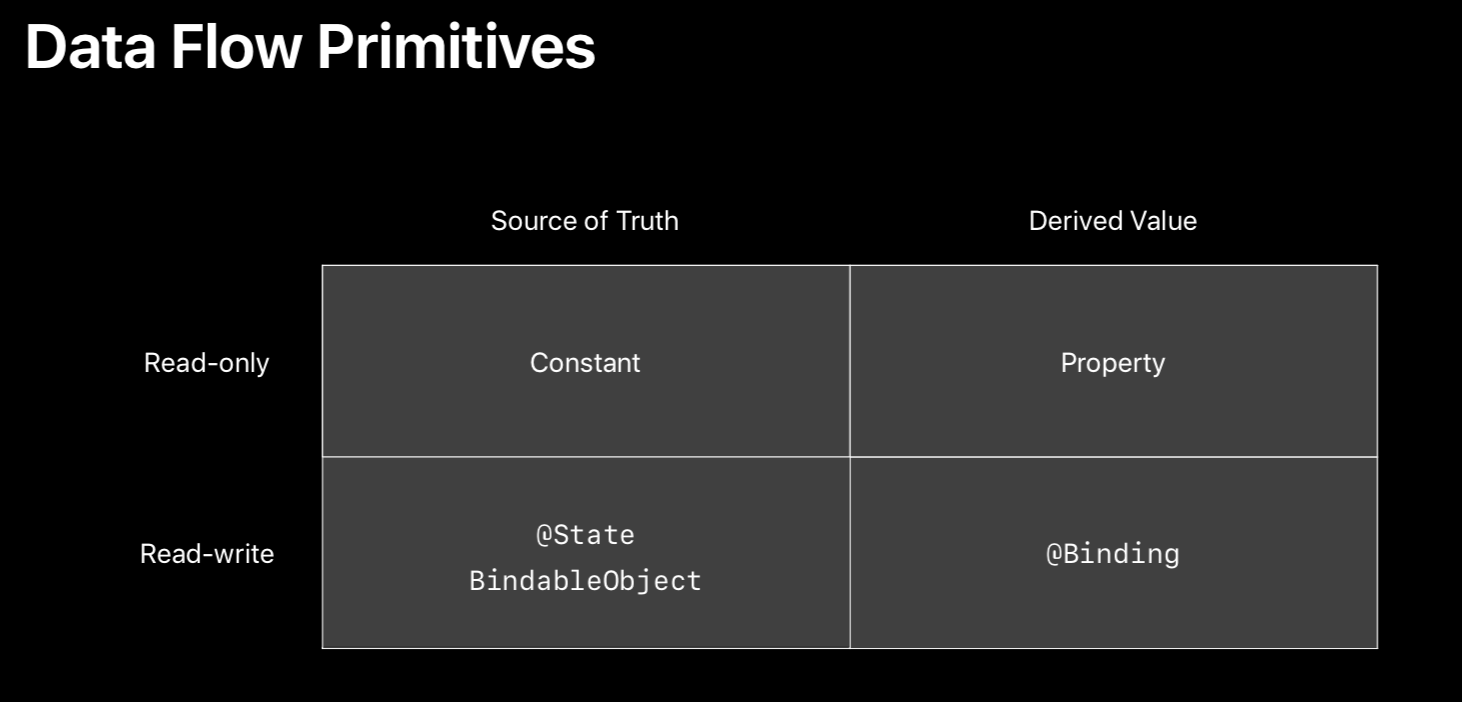
\includegraphics[width=1\textwidth]{images/DataFlowPrimitives.png}
\centering
\caption{\textit{Различити омотачи података}}
\label{slika:data_flow_primitives}
\end{figure}

% Dodati kod koji bolje objasnjava omotace podataka
\begin{lstlisting}[caption=\textit{{Омотачи података - State}}, label={lst:Омотачи података - State}, language=Swift, frame=single]
    struct Recept: View {
        var recept: ReceptPodatak
        @State private var daLiJeOmiljen: Bool = false
        
        var body: some View {
            VStack {
                Text(recept.ime)
                // 'OmiljenRecept' je pogled koji sadrzi zvezdicu koja oznacava da li je recept medju omiljenima (puna zvezdica - jeste, prazna - nije) 
                // Prosledjivanjem promenljive 'daLiJeOmiljen' uz prefiks '$' omogucava se promena promenljive 'daLiJeOmiljen' u pogledu 'OmiljenRecept'
                OmiljenRecept(daLiJe: $daLiJeOmiljen)
            }
        }
    }
\end{lstlisting}

\begin{lstlisting}[caption=\textit{{Омотачи података - Binding}}, label={lst:Омотачи података - Binding}, language=Swift, frame=single]
    struct Recept: View {
    // Promenljiva 'isPlaying' je definisana u jednom pogledu, a moze se menjati u drugom
    var recept: ReceptPodatak
    @Binding var daLiJeOmiljen: Bool

    var body: some View {
        Button(action: {
            // Akcija dugmeta koja menja promenljivu 'daLiJeOmiljen'
            self.daLiJeOmiljen.toggle()
        }) {
            // Provera promenljive 'daLiJeOmiljen' i prikaz odgovarajuce slike
            Image(systemName: daLiJeOmiljen ? "star.fill" : "star.empty")
        }
    }
}
\end{lstlisting}

\begin{lstlisting}[caption=\textit{{Омотачи података - Environment}}, label={lst:Омотачи података - Environment}, language=Swift, frame=single]
    struct Kulinarstvo_widgetEntryView : View {
    var entry: Provider.Entry
    
    // Citamo podatke za 'widgetFamily' iz okruzenja aplikacije (eng. Environment) i smestamo ih u promenljivu 'widgetFamily'
    @Environment(\.widgetFamily) var widgetFamily
    
    @ViewBuilder
    var body: some View {
        // U zavisnosti od promenljive 'widgetFamily' prikazujemo odgovarajuci widget
        switch widgetFamily {
        case .systemSmall:
            RecipeView(recipe: entry.recipe)
                .widgetURL(entry.recipe.url)
        case .systemMedium:
            RecipeMediumView(recipe: entry.recipe, ingredients: entry.recipe.ingredients.count > 3 ? Array(entry.recipe.ingredients.dropLast(entry.recipe.ingredients.count - 3)) : entry.recipe.ingredients)
        default:
            Text("")
        }
    }
}
\end{lstlisting}

\subsection{Разлика SwiftUI и UIKit}
\label{subsec:Разлика SwiftUI и UIKit}

\indent \textit{UIKit} и \textit{SwiftUI} су радна окружења развијена од стране \textit{Apple-а}, а који нам помажу приликом израде корисничког интерфејса апликације.
\\
\indent Генерално, највећа разлика између ова два радна окружења је у начину размишљања, како доћи до решења и како то решење касније имплементирати. Ову разлику ћемо најбоље показати на једном конкретном примеру; Форма за пријављивање на неки сајт, креирање вертикалног скупа елемената, хоризонтално и вертикално центрираних у том скупу, а скуп ће се састојати од два текстуална поља(за корисничко име и лозинку) и дугмета(са акцијом провере података).
\\
\indent Са \textit{UIKit-ом} морамо водити рачуна о свим ситним детаљима као што су: креирање вертикалног скупа елемената, његово додавање у главни поглед, креирање текстуалног поља, додавање текстуалног поља у скуп елемената, додавање аутоматског ограничења распореда како бисмо центрирали текстуално поље, понављање поступка за друго текстуално поље и поновно понављање поступка за дугме. 
\\ % можда кораке прабацити у листу, због прегледности
\indent За разлику од тога, као што смо напоменули, \textit{SwiftUI} се базира на декларативном начину програмирања, и овде је довољно да наведемо да желимо да групишемо два текстуална поља и дугме у вертиклани скуп елемената и у ком погледу желимо да се прикажу. Све ситне детаље ће радно окружење одрадити уместо нас онако како је то уобичајено дефинисано. Наравно не морамо се придржавати свих детаља које окружење одради, већ их можемо, по потреби, и сами мењати.
\\
\indent Уколико сагледамо архитектуре образаца, можемо приметити да се \textit{UIKit} првенствено базира на \textit{MVC}\footnote{Архитектурни образац Модел-Поглед-Контролер (енг. Model-View-Controller) који се заснива на подели на три целине, модел - структура података, поглед - приказ података у корисничком окружењу, контролор - управљање моделом} обрасцу, док за разлику од њега, \textit{SwiftUI} користи \textit{MVVM}\footnote{Архитектурни образац Модел-Поглед-Модел погледа (енг. Model-View-ViewModel) који се заснива на подели на три целине, модел - структура података, поглед - приказ података у корисничком окружењу, модел погледа - стање података у моделу} образац.
\\
\indent Креирање корисничког интерфејса у \textit{UIKit-у} коришћењем само \textit{Swift} кода је веома компликовано, и за веће пројекте готово немогуће, јер се мора водити рачуна о сваком детаљу. Најчешћи начин израде корисничког интерфејса је коришћењем \textit{Storyboards-а} i \textit{Interface Builder-а}, помоћу којих програмер креира кориснички интерфејс превлачењем, спустањем и конфигурацијом елемената. У \textit{SwiftUI-у} се кориснички интерфејс изграђује помоћу \textit{Swift} кода. Једноставно изјаснимо се шта желимо да направимо и радно окружење то уради за нас. Да би процес креирања био бржи и приступачнији, од верзије \textit{Xcode-а} 11, која је изашла у исто време када је представљен \textit{SwiftUI}, постоји могућност прегледа уживо сваког појединачног погледа који смо креирали или скупа више погледа одједном. О овоме ће бити више речи у поглављу \ref{subsec:Xcode - преглед уживо} - \nameref{subsec:Xcode - преглед уживо}.
\\
\indent За заинтересованије читаоце, постоји могућност комбиновања два радна окружења и коришћење \textit{SwiftUI-а} унутар \textit{UIKit} кода, или обратно, али ово остављам читаоцима да сами истраже како се то може постићи.

\subsection{Xcode - преглед уживо}
\label{subsec:Xcode - преглед уживо}

\indent Са представљањем \textit{SwiftUI-a}, \textit{Apple} је представио и нову верзију њиховог ИРО-а, \textit{Xcode11}, у коме је додато својство рада у новом радном окружењу као и могућност прегледа уживо сваког погледа. 
\\
\indent Предност оваквог начина писања кода је пре свега у могућности брзог прегледа измена кода и то без поновног обнављања (енг. rebuilding) апликације, поготово уколико радимо на додавању или измени погледа који се налази дубоко у навигацији апликације и за који нам је потребно више кликова и/или превлачења да бисмо до њега дошли. 
\\
\indent Преглед уживо нам још може помоћи да и у \textit{SwiftUI-у} користимо метод превлачење и пуштање за креирање корисничког интерфејса, који се разликује од претходног који смо користили унутар \textit{Storyboard-а}, јер сваки елемент превлачимо у део где пишемо код и када га испустимо тај елемент постане део нашег кода. 
% Слика превлачења и пуштања за SwiftUI

\indent Да бисмо омогућили коришћење приказа уживо постоје пар ствари које морамо претходно одрадити и оне ће бити приказане у коду.

\begin{lstlisting}[caption=\textit{{Xcode - преглед уживо}}, label={lst:Xcode - преглед уживо}, language=Swift, frame=single]
    // Strukturu 'PlaceholderView' koristimo za prikazivanje jednog od elemenata(u ovom slucaju prvog) iz liste u pregledu uzivo, sa podrazumevanim podacima
    struct PlaceholderView : View {
        var body : some View {
            Kulinarstvo_widgetEntryView(entry: SimpleEntry(date: Date(), configuration: ConfigurationIntent(), recipe: RecipeModel.testData[0]))
        }
    }
    
    // Struktura u kojoj konfigurisemo prikaz uzivo, mora implementirati protokol 'PreviewProvider'
    struct Kulinarstvo_widget_Previews: PreviewProvider {
        static var previews: some View {
            // Ukoliko zelimo vise prikaza odjednom, to mozemo uciniti tako sto cemo ih smestiti u jednu grupu
            Group {
                // Prikaz malog widget-a sa prvim elementom iz liste
                Kulinarstvo_widgetEntryView(entry: SimpleEntry(date: Date(), configuration: ConfigurationIntent(), recipe: RecipeModel.testData[0]))
                    .previewContext(WidgetPreviewContext(family: .systemSmall))
                
                // Prikaz srednjeg widget-a sa skrivenim sadrzajem, koji sluzi za prikaz widget-a bez konkretnog sadrzaja, na primer kako bi widget izgledao dok se podaci ucitavaju
                PlaceholderView()
                    .previewContext(WidgetPreviewContext(family: .systemMedium))
                    .redacted(reason: .placeholder)
            }
                
        }
    }    
\end{lstlisting}

\indent Након сваке измене коју направимо у коду који је везан за поглед(е) који се налази у прегледу уживо, \textit{Xcode} ће изнова направити нову верзију и покренути је у прозору за преглед уживо. Као што смо видели у примеру кода изнад, преглед уживо не мора приказивати само један поглед, већ можемо груписати колико год желимо различитих погледа и све их приказати одједном. Предност оваквог приступа је могућност истовременог прегледа, старог и новог изгледа погледа, више величина \textit{widget-а}, истих погледа са светлом и тамном бојом позадине, погледа на различитим језицима...

% Слика преглед уживо

\indent Ко жели више да истражи о овој теми, препоручујем да одгледа два одлична клипа са \textit{Apple-ове} конференције за програмере из 2019. и 2020. године респективно. Клипови су: \href{https://developer.apple.com/videos/play/wwdc2019/233/}{\textit{'Mastering Xcode Previews'}} и \href{https://developer.apple.com/videos/play/wwdc2020/10149/}{\textit{'Structure your app for SwiftUI previews'}}.

\chapter{Улога и развој Widget-a}

\section{Основно}

\indent \textit{Widget-и} на уређајима са \textit{Apple} платформом узимају један од кључних делова апликације за коју је развијени и приказују га крајњим корисницима тамо где ће га најлакше уочити, на \textit{iPhone-у} и \textit{iPad-у} се може налазити на почетном екрану или у делу \textit{Today View-а}, док се на \textit{Mac} уређајима налазе у центру за нотификације.
\\
\indent Величина \textit{widget-а} није флексибилна као на \textit{Android} уређајима, па тако постоји могућност креирања малих (величина 2x2 места на почетном екрану \textit{iPhone-а}), средњих (2x4), великих (4x4) и од верзије \textit{iPadOS15} екстра великих (4x8), само за \textit{iPad} уређаје, \textit{widget-а}. 
\\
\indent Скуп свих тренутно доступних \textit{widget-а} на уређају налази се у галерији \textit{widget-а} (енг. widget gallery), која помаже корисницима приликом одабира конкретне величине и типа \textit{widget-а} (Једна апликација може испоручити више типова \textit{widget-а} исте величине). Унутар галерије такође постоји опција за измену \textit{widget-а}, у којој корисници могу да контролишу и мењају своје \textit{widget-е}, и тиме их што више прилагоде себи, али само уколико је то у току конструисања \textit{widget-а} од стране програмера то омогућено. Више речи о овоме биће у делу \ref{sec:Развој Widget-a} - \nameref{sec:Развој Widget-a}.
\\
\indent На \textit{iOS} и \textit{iPadOS} системима, галерија има могућност додавања паметних гомила (енг. smart stack), који могу садржати до 10 различитих \textit{widget-а} исте величине. Паметна гомила приказује само један од \textit{widget-а} који се налазе у њој. Корисник може сам да мења који ће \textit{widget} бити приказан једноставним померањем (енг. scrolling). Временом, паметна гомила може научити који \textit{widget} корисник ставља на почетак гомиле у току дана (или недеље) и сама мењати примарне \textit{widget-е} у одређеном тренутку (на пример, након гашења аларма, прво се приказује \textit{widget} са временском прогнозом, па најновије вести, гужва у саобраћају...)
\\
\indent \textit{Siri}\footnote{Интелигентни лични асистент на уређајима са \textit{Apple} платформом} може и сама додати \textit{widget-е} у паметну гомилу, уколико претпостави да постоји неки \textit{widget} који би кориснику био користан. Након тога, корисник сам одлучује да ли жели да новододати \textit{widget} остане у паметној гомили или не.

\subsection{WidgetKit}
\indent \textit{WidgetKit} је радно окружење, које уз \textit{widget API} из  \textit{SwiftUI-а} служи за израду \textit{widget-а}, од његовог изгледа, преко временског ажурирања па све до омогућавања конфигурације \textit{widget-а} од стране крајњих корисника и управљања паметном гомилом приликом ротације \textit{widget-а} од стране самог система. 
\\
\indent Још једна ствар коју ово радно окружење пружа је повезивање апликације и самог \textit{widget-а}, што омогућава кориснику да отвори апликацију и аутоматски оде на одговарајући поглед из \textit{widget-а} када жели да види детаљније податке. Пажња код ових ствари је да \textit{widget} не би смео да служи само као пречица за покретање апликације, више о томе биће објашњено у делу \ref{sec:Дизајн Widget-a} - \nameref{sec:Дизајн Widget-a}.


\section{Развој Widget-a}
\label{sec:Развој Widget-a}
\indent \textit{Widget} је ништа друго до заправо само један \textit{SwiftUI} поглед. \textit{Widget-и} су тренутно једини део \textit{Apple} оперативних система који у потпуности морају бити написани коришћењем \textit{SwiftUI} радног оквира. \textit{Apple} је отпочетка развоја \textit{widget-а} имао на уму овакву идеју, због начина приказивања података, повременог ажурирања података и немогућности корисничке интеракције са самим \textit{widget-има} (осим једноставног клика којим се отвара одређени део аплиакције).  
\\
\indent Додавање \textit{widget-а} у апликацију и његово конфигурисање је веома лако и биће приказано по ставкама у наставку ове секције. 

\subsection{Додавање widget додатка у апликацији}
\indent Шаблон за \textit{widget} додатак креира основне ставке потребне за његову израду. Унутар овог додатка се креирају сви потребни \textit{widget-и} за апликацију, не зависно од њиховог броја и величине. У посебним ситуацијама, различити \textit{widget-и} могу бити одвојени у посебним додатцима, ово се најчешће односи када један тип \textit{widget-а} захтева одређене дозволе од стране корисника, док за други тип оне нису потребне (на пример, приступ тренутној локацији корисника).

\indent Кораци за креирање \textit{widget} додатка:
\begin{enumerate}
    \item Отворити пројекат у \textit{Xcode-u} и изабрати \textit{File -> New -> Target}
    % slika
    \item Из групе \textit{Application Extension}, изабрати \textit{Widget Extension} и кликнути \textit{Next}
    % slika
    \item Унети име додатка
    % slika
    \item Уколико ће \textit{widget} подржавати конфигурацију од стране корисника, штиклирати поље \textit{Include Configuration Intent}
    % slika
    \item Кликнути на \textit{Finish}
    % slika
\end{enumerate}

\subsection{Додавање детаља конфигурације}
\indent Као што смо већ рекли, шаблон \textit{widget} додатка пружа иницијалну имплементацију \textit{widget-а} која имплементира \textit{Widget} протокол. Два могућа начина конфигурације \textit{widget-а} су статичка (енг. StaticConfiguration) и конфигурација са сврхом (енг. IntentConfiguration).
\indent Статичка конфигурација се користи за \textit{widget-е} који немају параметре који могу бити конфигурисани од стране корисника (на пример, системска апликација \textit{Screen time} која води статистику о времену проведеном на одговарајућем уређају).
\indent Конфигурација са сврхом се користи за \textit{widget-е} чији одређени параметри могу бити конфигурисани од стране корисника (на пример, системаска аплиакција за временску прогнозу, где корисник може наместити одређени град за који жели да добија податке). Ова конфигурација ће бити укључена и конфигурациони фајл ће бити додат уколико је корисник приликом додавања \textit{widget} додатка, штиклирао поље \textit{Include Configuration Intent}.
\\
\indent Да би програмер спровео почетну конфигурацију \textit{widget-а} потребно је да проследи следеће параметре:
\begin{itemize}
    \item Тип (енг. Kind), стринг који идентификује \textit{widget}, требао би да казује шта \textit{widget} представља
    \item Снабдевач (енг. Provider), објекат класе која имплементира \textit{TimelineProvider} протокол и кроз временску линију коју проиводи одређује у ком тренутку ће \textit{widget} бити поново изрендерован и нови подаци бити приказани. Више о овом протоколу и свеукупној причи о временој линији у делу \ref{subsec:Временска линија} - \nameref{subsec:Временска линија}
    \item Затворење садржаја (енг. Content Closure), затворење које садржи \textit{SwiftUI} поглед и које \textit{WidgetKit} позива када дође време за поновно рендеровање садржаја \textit{widget-а}
    \item Прилагођена сврха (енг. Custom Intent), фајл који дефинише параметре које корисник може мењати и прилагођавати себи. Више о овоме: \ref{subsec:Intent} - \nameref{subsec:Intent}
\end{itemize}
% Kod za pocetnu konfiguraciju widget-a, uz dodatne parametre, ime za prikaz, opis, velicine widget-a, boja pozadine widget-a

\subsection{Временска линија}
\label{subsec:Временска линија}
\indent Снабдевач временске линије генерише временску линију која се састоји од уноса (енг. entries), а сваки унос садржи датум и време када је потребно ажурирати садржај \textit{widget-а}. Када се датум и време из уноса подударе са реалним временом, \textit{WidgetKit} позива затворење садржаја које потом приказује ажуриране податке. 
\\
\indent Да би \textit{widget} био приказан у \textit{widget} галерији, \textit{WidgetKit} захтева од снабдевача преглед снимка (енг. Preview snapshot). Дохватање прегледа снимка се разрешава провером променљиве \textit{isPreview} којом се проверава да ли снабдевач прегледа снимка шаље тренутни снимак за приказ у галерији или за приказ \textit{widget-а} на почетном екрану (или \textit{Today} погледу, или центру за обавештења). Када је параметар \textit{isPreview} тачан, \textit{widget} се приказује у галерији. Уколико за приказ \textit{widget-а} треба да буду приказани и одређени подаци, а подаци нису пристигли са серверске стране, постоје два решења. Можемо приказати подразумеване, унапред одређене податке, или можемо користити податке које чувају место правим подацима (енг. placeholder). 
% Слика са placeholder podacima i objasnjenje kroz komentare
\\
\indent Када пристигну подаци са сервера, снабдевач добија обавештење, сакупља реалне податке и приказује \textit{widget} са њима.
\\
\indent Након што корисник дода \textit{widget} на почетни екран и буде приказан иницијални снимак изгледа \textit{widget-а}, \textit{WidgetKit} позива функцију \textit{getTimeline} из провајдера, чиме захтева временску линију.
% Primer sa ovom funkcijom iz koda

\subsection{Intent}
\label{subsec:Intent}
\indent \textit{Widget-i} предтављају погледе који не интерагују са корисницима, односно не подржавају интерактивне елементе, као што су \textit{scroll} поглед и \textit{switch} дугме. Уколико желимо да допустимо једну врсту интеракције корисника са \textit{widget-ом} можемо омогућити конфигурацију \textit{widget-а} од стране корисника, коришћењем \textit{Intent} конфигурације, у којој наводимо све параметре које корисник може да промени (и дозвољене вредности за те параметре). 
\\
\indent Да би додали параметре које корисник може да конфигурише, постоје предуслови које морамо испунити:
\begin{itemize}
    \item Додавање дефиниције \textit{intent-а}, који дефинише конфигурабилне параметре 
    \item Коришћење \textit{IntentTimelineProvider} протокола за провајдера временска линије, уместо \textit{TimelineProvider}, да би конфигурација параметара од стране корисника била сачувана у уносима временске линије
    \item Уколико параметри зависе од динамичких података, потребно је имплементирати екстензију \textit{intent-а}
\end{itemize}
% Слике додавања intent-a и његова конфигурација, примери кода и приказ конфигурације параметара у симулатору

\subsection{Везе унутар \textit{widget-а}}
\indent Једини начин директне комуникације између корисника и \textit{widget-а}, остварена је везама (енг. links) унутар \textit{widget-а}. Када корисник кликне на \textit{widget} отвара се апликација којој тај \textit{widget} припада, и можемо конфигурисати који део апликације желимо да прикажемо кориснику у зависности од елемента унутар \textit{widget-а} на који је корисник кликнуо. 
\\ 
\indent Свим величинама \textit{widget-а} може бити додат \textit{widgetURL(\_:)} модификатор, којим се одређује у који део апликације ће корисник бити одведен када кликне на \textit{widget}.
\\
\indent За све величине \textit{widget-а}, осим малих, могу се користити и везе које су додате једном елементу унутар \textit{widget-а} и којим је одређено место у апликацији које ће бити отворено (на пример, један \textit{widget} средње величине, који садржи листу са 3 рецепата, сваки елемент листе има везу која води ка детаљној страни о рецепту који тај елемент представља). Иако \textit{widget} користи везе унутар својих елемената, може користити и модигикатор \textit{widgetURL(\_:)} из претходног примера. Овај модификатор ће бити активиран уколико корисник кликне на елеменат у \textit{widget-у} који нема дефинисану везу. 
% Примери кода

\subsection{Више \textit{widget-а} у једном проширењу}
\indent Уколико желимо да користимо више различитих типова \textit{widget-а} у једном проширењу, то можемо лако урадити уз само пар измена главног дела проширења, означеног атрибутом \textit{@main}. 

\begin{lstlisting}[caption=\textit{{Више widget-а у једном проширењу}}, label={lst:Више widget-а у једном проширењу}, language=Swift, frame=single]
    @main
    // Umesto protokola 'Widget', koristimo 'WidgetBundle'
    struct ReceptiWidgets: WidgetBundle {
        // Definisemo atribut '@WidgetBundlerBuilder'
        @WidgetBundleBuilder
        // Definisemo telo, koje ovog puta implementira protokol 'Widget'
        var body: some Widget {
            DetaljanPrikazReceptaWidget()
            ListaRecepataWidget()
            SpisakZaKupovinuWidget()
        }
    }
\end{lstlisting}

\section{Дизајн Widget-a}
\label{sec:Дизајн Widget-a}

\subsection{Фокус Widget-a}
\indent Главна улога \textit{widget-а} је приказивање садржаја који кориснику пружа корисне информације без покретања апликације. Подаци које приказује треба да буду минималистички, да одговарају величини \textit{widget-а} (већа величина треба да повлачи и већу количину података) и да буду временски и кориснички релевантни. Први корак у дизајну \textit{widget-а} је избор једног дела аплиакције, који ће тај \textit{widget-а} да представља. 
\\
\indent Свака величина \textit{widget-а} која је омогућена за додавање из галерије, треба да садржи одређену количину информација која је пропорционална тој величини. Никако не смемо допустити да више величина \textit{widget-а} приказују исте податке, али истовремено приликом додавања нових података, морамо водити рачуна о почетној идеји, односно делу апликације које тај \textit{widget} треба да представља. Уколико немамо довољну количини података за веће \textit{widget-е} (на пример, за \textit{widget} величине \textit{large}), можемо једноставно забранити ту величину за тај тип \textit{widget-а}. % Мало боље објашњење
\\
\indent \textit{Widget} не би смео да служи само као пречица за покретање аплиакције. Корисници очекује од сваког \textit{widget-а} да им покаже корисне информације, у супротном неће наићи на добар одзив, и истовремено може и штетити самој апликацији (мањи број корисника, лошија оцена у продавници).

\subsection{Ажурни подаци}
\indent Да би \textit{widget-и} могли да пружају корисне и прецизне информације у скоро сваком тренутку, морају повремено бити ажурирани. \textit{Widget-и} не подржавају ажурирање у реалном времену, а и сам систем може ограничити ажурирање \textit{widget-а} у завиности од корисничког понашања и интеракције са њим, па се морамо потрудити да нађемо начин на који ће подаци у нашем \textit{widget-у} увек бити релевантни. 
\\
\indent Потребно је пронаћи оптимално време за ажурирање података у \textit{widget-у}, узимајући у обзир колико се сами подаци често мењају и колико често корисницима може бити корисно да виде те податке. Уколико након публикације \textit{widget-а} уочимо да су корисницима чешће или ређе потребни новији подаци, можемо променити време између два ажурирања и тиме побољшати корисничко искуство. Још једна корисна ствар код информација које су временски зависне (на пример, тренутно стање неког индекса или акције на берзи), можемо у \textit{widget-у} додати и поље које ће представљати датум  и време када су подаци последњи пут ажурирани.
\\
\indent Иако не можемо да приказујемо податке у реалном времену, за неке податке можемо искористити помоћ система за одређивање датума и времена, па тако уколико би имали \textit{widget} који приказује време у које ће се огласити аларм, истовремено можемо имати и ажуран податак о томе колико је времена остало до оглашавања аларма.  

\subsection{Конфигурабилност и интеракција}
\indent У већини случајева \textit{widget} треба да омогући кориснику конфигурабилност како би пружио корисне информације (на пример, књига коју корисник тренутно чита и његов прогрес у апликацији \textit{Apple Books}), док поједине апликације могу то да изоставе (на пример, најновије вести). 
\\
\indent Уколико желите да ваш \textit{widget} буде конфигурабилан, потрудите се да подешавања буду што једноставнија и не тражите превише информација од корисника. Кориснички интерфејс за измену \textit{widget-а} је унапред одређен и исти за све, као што смо показали у делу \ref{subsec:Intent} - \nameref{subsec:Intent}.
\\
\indent Када корисник кликне на \textit{widget} или део унутар њега, за веће величине, очекује да буде одведен на жељену страницу, да не мора да претражује и даље апликацију (на пример, када кликне на одређени рецепт у \textit{widget-у}, желеће да му се отвори страница са детаљним приказом тог рецепта, а не почетна страна). Истовремено, треба се избећи превише веза на малом простору, где се лако може десити да због густине распореда, корисник кликне грешком на један елемент, а желео је да притисне сасвим други.

\subsection{Дизајн прилагођен свима}
\indent \textit{Widget-и} треба да имају јарке боје како би се истицали на екрану, али истовремено и јасно видљив текст како би корисник могао да види све потребне информације "бацањем погледа" након откључавања или непосредно пре закључавања уређаја. Трудите се да \textit{widget} прилагодите свом бредну или својој апликацији (боје, фонт текста, јединствени елементи...). Водите рачуна да истовремено не претерате са обележјима, корисницима веома често није потребно да виде лого ваше компаније да би препознали о ком се \textit{widget-у} ради, док истовремено вам заузима место и смањује простор за приказ важних података, нарочито на малој величини \textit{widget-а}.  
\\
\indent Када сагледамо количину информација коју желимо да прикажемо у \textit{widget-у}, морамо бити оптимални. Уколико прикажемо премало информација, \textit{widget} неће имати превелики значај за кориснике, док превише информација на мало простора отежава читање и разумевање података.
\\
\indent Једна од битнијих ствари коју не смемо заборавити, поготово у данашње време, је дизајн \textit{widget-а} за обе врсте боја системске позадине (светле и тамне). Дизајн оба \textit{widget-а} се не сме разликовати од системске боје позадине, јер ниједан корисник не жели видети таман текст на светлој боји позадине уколико је изабрао тамну системску боју позадине. Приликом израде обе врсте дизјна нам може помоћи \textit{Xcode preview} који омогућава да истовремено сагледамо оба дизајна, међусобно их упоредимо и исправимо евентуалне недостатке.
\\
\indent \textit{Apple} саветује да се никад не користи фонт текста мањи од 11 поена\footnote{\textit{Apple-ов} израз за "број који треба уписати у поље", универзална мера у дизајну на \textit{Apple} платформама}. Коришћење мањег фонта би корисницима знатно отежало употребу \textit{widget-а} и дефинитивно смањило број корисника. Поред овога, увек се требају користити званични елементи за приказ текста, како би се омогућила скалабилност као и системско читање текста. 
\\
\indent Потребно је да се добро покажете већ на првом кораку, зато посебну пажњу треба обратити на дизајн прегледа \textit{widget-а} унутар галерије, за све типове и величине који ваш \textit{widget} подржава, као и приказ чувара места уместо реалних података уколико они нису пристигли на време са сервера и немате подразумеване податке. 
\\
\indent Уколико имате елементе у својој апликацији који се истовремено налазе и на \textit{widget-у} постарајте се да имају исту функционалност, јер бисте у супротном само збунили кориснике. 
\\
\indent Искористите могућност приказивања описа \textit{widget-а} у галерији и саставите кратак и јасан опис функционалности вашег \textit{widget-а}. Такође, групишите све величине једног типа \textit{widget-а} са јединственим описом.
\\
\indent Обратите пажњу на скалабилност елемената унутар \textit{widget-а}. Систем аутоматски прилагођава величину вашег \textit{widget-а} величини екрана уређаја, зато будите пажљиви приликом додавања елемената. Најбоље је користити проверене елементе који пружају флексибилност, у овом случају било који основни \textit{SwiftUI} елемент, или њихова комбинација.

\chapter{Опис апликације}

\chapter{Закључак}

\literatura

\end{document}
